\documentclass[aspectratio=169,11pt]{beamer}
\usepackage[T1]{fontenc}
\usepackage{lmodern,amsmath,amssymb,mathtools,bm,booktabs,array,graphicx,tikz}
\usetikzlibrary{arrows.meta,positioning,calc,decorations.pathreplacing,patterns}
\definecolor{ink}{HTML}{17344D}\definecolor{accent}{HTML}{087E8B}\definecolor{pale}{HTML}{EDF5F5}\definecolor{gold}{HTML}{AD6B19}
\providecommand{\dd}{\,\mathrm{d}}\providecommand{\R}{\mathbb{R}}
\providecommand{\E}{\mathbb{E}}\providecommand{\Var}{\operatorname{Var}}
\providecommand{\Cov}{\operatorname{Cov}}\providecommand{\diag}{\operatorname{diag}}
\providecommand{\norm}[1]{\left\lVert#1\right\rVert}
\providecommand{\abs}[1]{\left|#1\right|}
\usefonttheme{professionalfonts}
\setbeamercolor{normal text}{fg=black,bg=white}
\setbeamercolor{frametitle}{fg=ink,bg=white}
\setbeamercolor{title}{fg=ink}\setbeamercolor{structure}{fg=accent}
\setbeamercolor{block title}{fg=ink,bg=pale}\setbeamercolor{block body}{fg=black,bg=pale!40}
\setbeamercolor{alerted text}{fg=accent}
\setbeamerfont{frametitle}{size=\Large,series=\bfseries}
\setbeamerfont{title}{size=\LARGE,series=\bfseries}
\setbeamertemplate{navigation symbols}{}
\setbeamersize{text margin left=.7cm,text margin right=.7cm}
\setbeamertemplate{frametitle}{\vspace{.18cm}\insertframetitle\par\vspace{.1cm}{\color{accent}\hrule height .6pt}\vspace{.12cm}}
\newcommand{\notestarget}{notes.pdf}\newcommand{\noteslabel}{Notes}
\setbeamertemplate{footline}{\hspace{.7cm}\color{ink}\scriptsize Scientific Computing in Python\quad\href{\notestarget}{\noteslabel}\hfill\insertframenumber\,/\,\inserttotalframenumber\hspace{.7cm}\vspace{.18cm}}
\setbeamercovered{invisible}
\hypersetup{pdfauthor={Zan Ahmad},pdftitle={Logistic regression and a neural-network classifier},pdfpagemode=UseNone}
\begin{document}
\begin{frame}[plain]\vfill
{\small\color{accent} Scientific Computing in Python \quad Lecture 6}\par\medskip
{\raggedright\hyphenpenalty=10000\exhyphenpenalty=10000\LARGE\bfseries\color{ink} Logistic regression and a neural-network classifier}\par\bigskip
Zan Ahmad\par\smallskip
{\small Winter 2026}\par\vfill\end{frame}
\renewcommand{\notestarget}{notes.pdf\#note-logistic-scores}
\begin{frame}[t,fragile,label=slide-logistic-scores]{Logistic scores}
\[
p_i=\sigma(a_i)=\frac1{1+e^{-a_i}},\qquad a_i=x_i^{\mathsf T}w+b.
\]
\pause{}
\[
\log\frac{p_i}{1-p_i}=a_i.
\]
\end{frame}
\renewcommand{\notestarget}{notes.pdf\#note-logistic-scores}
\begin{frame}[t,fragile,label=slide-threshold-geometry]{Threshold geometry}
\[
p_i\geq\frac12\iff a_i\geq0.
\]
\pause{}
Changing the threshold changes the decision rule. It does not change the fitted score surface.
\end{frame}
\renewcommand{\notestarget}{notes.pdf\#note-bernoulli-negative-log-likelihood}
\begin{frame}[t,fragile,label=slide-bernoulli-negative-log-likelihood]{Bernoulli negative log likelihood}
\[
\ell_i=-y_i\log p_i-(1-y_i)\log(1-p_i)
=\log(1+e^{a_i})-y_ia_i.
\]
\pause{}
\begin{verbatim}
loss = np.mean(np.logaddexp(0, logits)-y*logits)
\end{verbatim}
\end{frame}
\renewcommand{\notestarget}{notes.pdf\#note-bernoulli-negative-log-likelihood}
\begin{frame}[t,fragile,label=slide-the-logit-derivative]{The logit derivative}
\[
\frac{\partial\ell_i}{\partial a_i}=\sigma(a_i)-y_i=p_i-y_i.
\]
\pause{}
\[
\nabla_wL=\frac1nX^{\mathsf T}(p-y).
\]
This simple residual drives the parameter update.
\end{frame}
\renewcommand{\notestarget}{notes.pdf\#note-gradient-descent-and-regularization}
\begin{frame}[t,fragile,label=slide-gradient-descent-and-regularization]{Gradient descent and regularization}
\[
L(w,b)=\frac1n\sum_i\ell_i+\frac\lambda2\|w\|_2^2.
\]
\pause{}
\[
w\leftarrow w-\eta\left[\frac1nX^{\mathsf T}(p-y)+\lambda w\right].
\]
\end{frame}
\renewcommand{\notestarget}{notes.pdf\#note-a-nonlinear-hidden-layer}
\begin{frame}[label=slide-linear-and-nonlinear-decision-boundaries-figure]{Linear and nonlinear decision boundaries}
\centering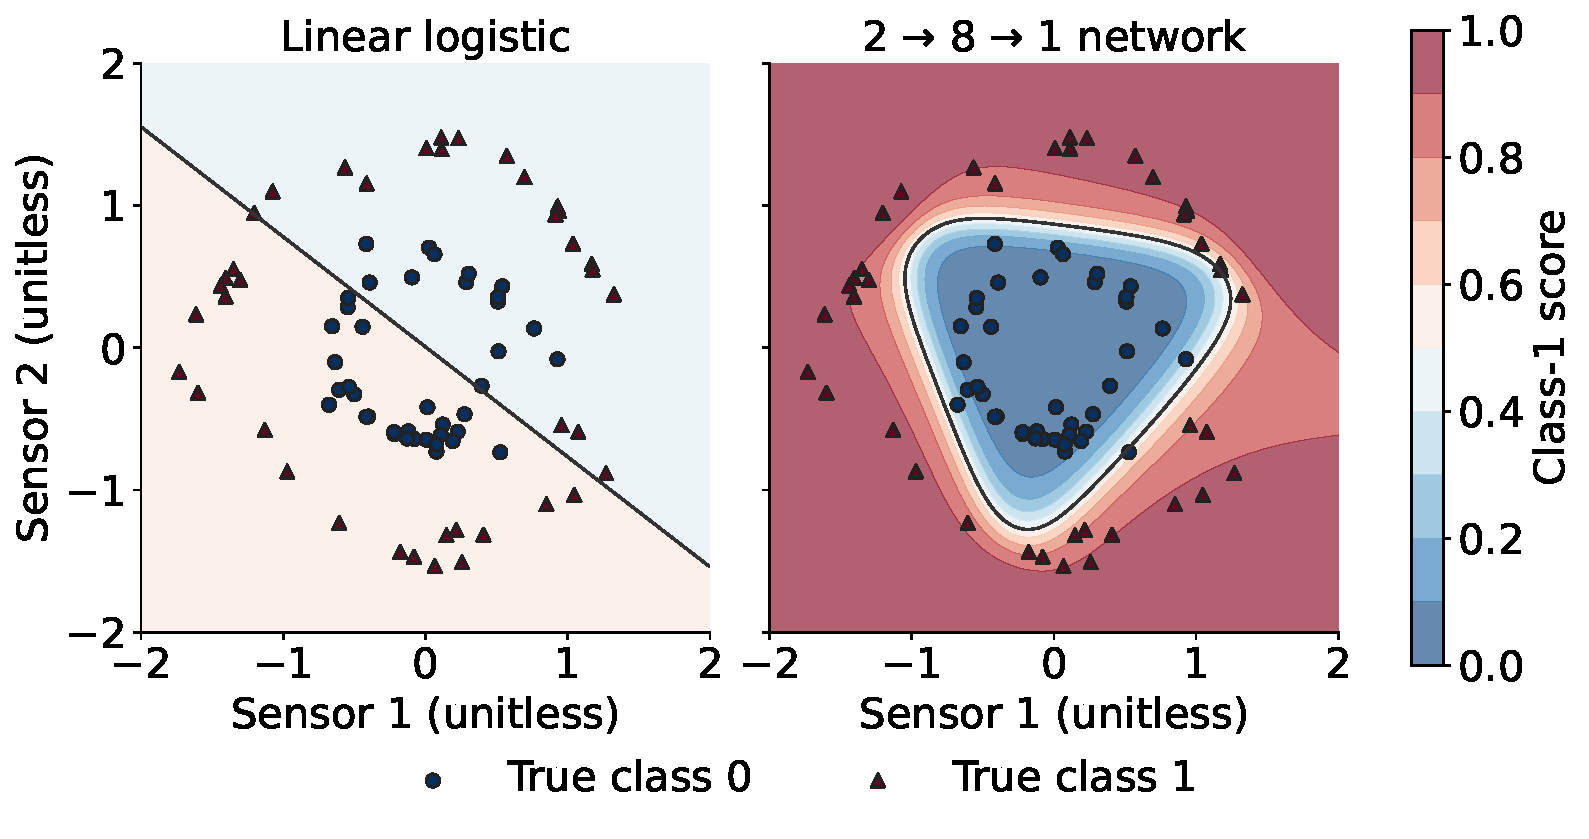
\includegraphics[width=.98\linewidth,height=.69\textheight,keepaspectratio]{decision-comparison.pdf}\end{frame}
\renewcommand{\notestarget}{notes.pdf\#note-gradient-descent-and-regularization}
\begin{frame}[t,fragile,label=slide-intercept-update]{Intercept update}
With no penalty on the intercept,
\[
b\leftarrow b-\eta\frac1n\sum_i(p_i-y_i).
\]
\pause{}
The choice of which parameters receive a penalty belongs to the objective definition.
\end{frame}
\renewcommand{\notestarget}{notes.pdf\#note-a-nonlinear-hidden-layer}
\begin{frame}[t,fragile,label=slide-a-nonlinear-hidden-layer]{A nonlinear hidden layer}
\[
H=\tanh(XW_1+b_1),\qquad a=Hw_2+b_2,\qquad p=\sigma(a).
\]
\pause{}
Shapes: $(n\times d)(d\times h)=n\times h$, then $(n\times h)(h\times1)=n\times1$.
\end{frame}
\renewcommand{\notestarget}{notes.pdf\#note-a-nonlinear-hidden-layer}
\begin{frame}[t,fragile,label=slide-backpropagation-through-tanh]{Backpropagation through tanh}
Let $D=(p-y)/n$. Then
\[
\nabla_{w_2}L=H^{\mathsf T}D,
\quad
D_1=(Dw_2^{\mathsf T})\odot(1-H^2).
\]
\pause{}
\[
\nabla_{W_1}L=X^{\mathsf T}D_1.
\]
Weight-penalty derivatives are added separately.
\end{frame}
\renewcommand{\notestarget}{notes.pdf\#note-confusion-counts}
\begin{frame}[t,fragile,label=slide-confusion-counts]{Confusion counts}
\[
\mathrm{accuracy}=\frac{TP+TN}{N},\quad
\mathrm{precision}=\frac{TP}{TP+FP},\quad
\mathrm{recall}=\frac{TP}{TP+FN}.
\]
\pause{}
Each denominator specifies a different reference group.
\end{frame}
\renewcommand{\notestarget}{notes.pdf\#note-a-controlled-model-comparison}
\begin{frame}[label=slide-training-loss-and-held-out-counts-figure]{Training loss and held-out counts}
\centering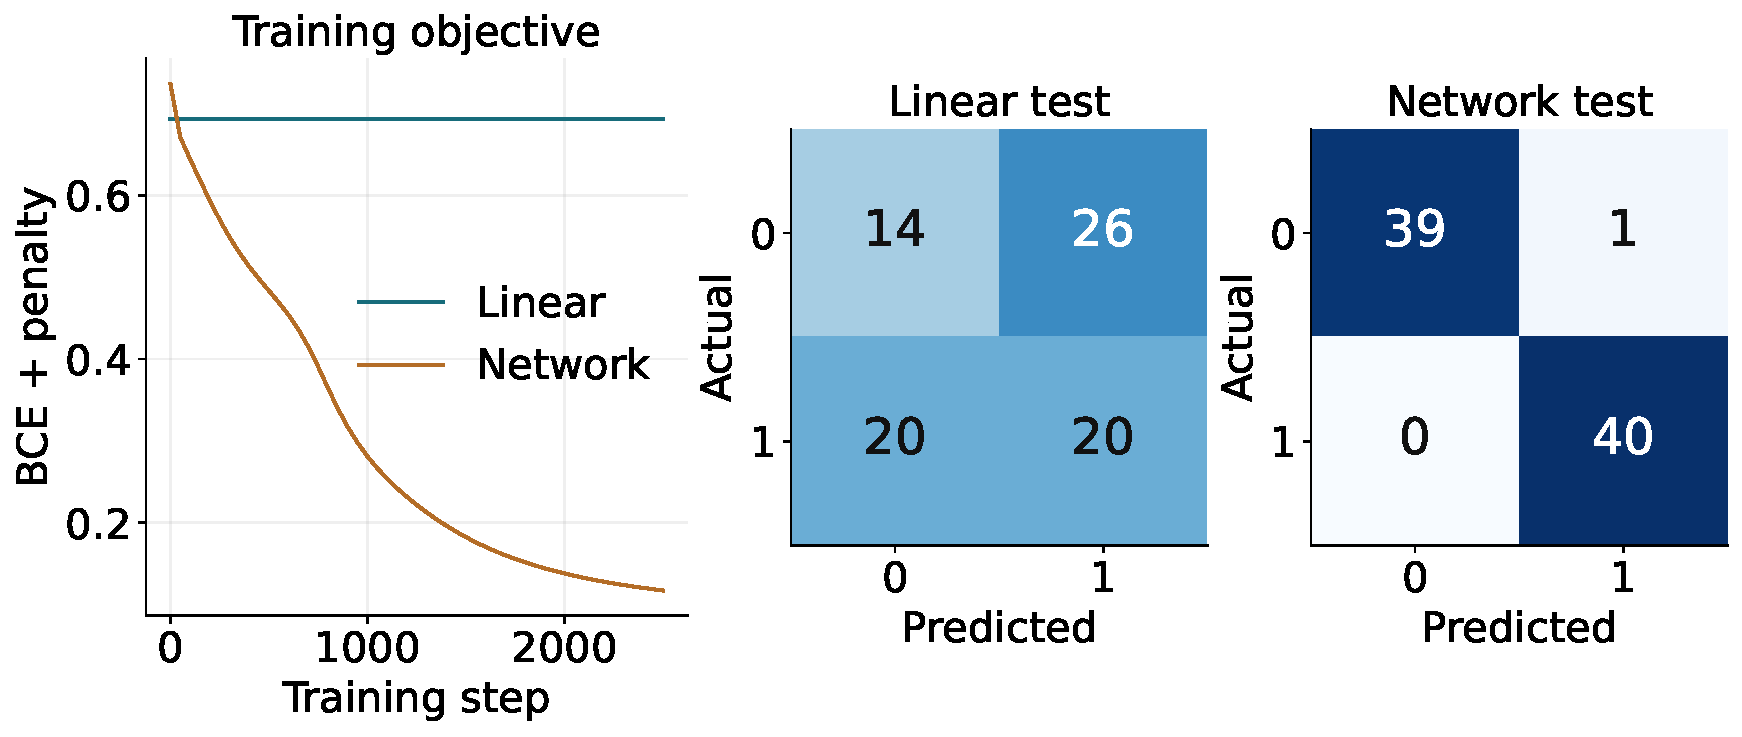
\includegraphics[width=.98\linewidth,height=.69\textheight,keepaspectratio]{loss-and-confusion.pdf}\end{frame}
\renewcommand{\notestarget}{notes.pdf\#note-confusion-counts}
\begin{frame}[t,fragile,label=slide-a-worked-confusion-matrix]{A worked confusion matrix}
\[
\begin{array}{c|cc}&\widehat y=0&\widehat y=1\\\hline y=0&30&10\\y=1&5&35\end{array}
\]
\pause{}
Accuracy $=65/80$, precision $=35/45$, recall $=35/40$. This illustrative matrix is separate from the companion's computed result.
\end{frame}
\renewcommand{\notestarget}{notes.pdf\#note-a-controlled-model-comparison}
\begin{frame}[t,fragile,label=slide-a-controlled-model-comparison]{A controlled model comparison}
Both classifiers receive the same feature representation and the same training rows.
\pause{}
The held-out comparison measures the consequences of the fitted functions, not differences in which test observations were selected.
\end{frame}
\renewcommand{\notestarget}{notes.pdf\#note-a-controlled-model-comparison}
\begin{frame}[t,fragile,label=slide-reproducibility-and-variability]{Reproducibility and variability}
A fixed seed reproduces one random split and initialization.
\pause{}
It does not quantify variation over other samples. Repeated, properly separated experiments are needed to study that variation.
\end{frame}
\end{document}
